\documentclass[12pt]{amsart}
%%%%%%%%%%%%%%%%%%%%%%%%%%%%%%%%%%%%%%%%%%%%%%%%%%%%%%%%%%%%%%%%%%%%%%%%%%%%%%%%%%%%%%%%%%%%%%%%%%%%%%%%%%%%%%%%%%%%%%%%%%%%%%%%%%%%%%%%%%%%%%%%%%%%%%%%%%%%%%%%%%%%%%%%%%%%%%%%%%%%%%%%%%%%%%%%%%%%%%%%%%%%%%%%%%%%%%%%%%%%%%%%%%%%%%%%%%%%%%%%%%%%%%%%%%%%   
\usepackage{amssymb}
\usepackage{amsmath}  
\usepackage{amsfonts}
\usepackage{mathrsfs}  
\usepackage{graphicx}
\usepackage{color}   
\usepackage[onehalfspacing]{setspace}
\usepackage{ragged2e}  
\justifying     
\usepackage{caption} 
\usepackage{etex} 
\usepackage{longtable} 
\usepackage{graphicx} 
\usepackage{amsmath}
\usepackage{multirow}
\usepackage{setspace}
\usepackage{footmisc}
\usepackage{amssymb}
\usepackage{amsfonts}
\usepackage[font=bf, justification=centering]{caption}
\usepackage{geometry}
\usepackage{float}
\usepackage{verbatim}
\usepackage{array}
\usepackage{booktabs}
\usepackage{pdflscape}
%\usepackage{xy} 
\usepackage{rotating}
\usepackage[round,authoryear]{natbib}
\usepackage{appendix}
\usepackage{lscape}
\usepackage{subcaption}
\usepackage{graphicx}
\usepackage{amsfonts}
\usepackage{placeins}
\usepackage[utf8]{inputenc}
\usepackage{charter}
\usepackage[colorlinks=true,citecolor=blue,urlcolor=blue,pdfpagemode=UseNone,pdfstartview=FitH]{hyperref}
\usepackage{apptools}
%\usepackage{chngcntr}
\usepackage{multibib}
\usepackage{multirow}
\DeclareUnicodeCharacter{00A0}{'}
%\usepackage[capposition=top]{floatrow}
\newcites{main,supp}{References,References}
%\AtAppendix{\counterwithin{lemma}{section}}
\makeatletter
\def\section{\@startsection{section}{1}
	\z@{1.0\linespacing\@plus\linespacing}{.5\linespacing}{\Large}}

\def\subsection{\@startsection{subsection}{2}
	\z@{.8\linespacing\@plus.7\linespacing}{.7\linespacing}{\large}}

\def\subsubsection{\@startsection{subsubsection}{3}
	\z@{.5\linespacing\@plus.7\linespacing}{-.5em}{\normalfont\bfseries}}
\makeatother                   

\setcounter{MaxMatrixCols}{10}
%TCIDATA{OutputFilter=LATEX.DLL}
%TCIDATA{Version=5.50.0.2953}
%TCIDATA{Codepage=936}
%TCIDATA{<META NAME="SaveForMode" CONTENT="1">}
%TCIDATA{BibliographyScheme=Manual}
%TCIDATA{LastRevised=Friday, May 08, 2015 15:13:41}
%TCIDATA{<META NAME="GraphicsSave" CONTENT="32">}
%TCIDATA{Language=American English}

\numberwithin{equation}{section}

\newtheorem{theorem}{Theorem}[section]
\newtheorem{lemma}{Lemma}[section]
\newtheorem{corollary}{Corollary}[section]
\theoremstyle{definition}
\newtheorem{definition}{Definition}[section]

\theoremstyle{definition}
\newtheorem{assumption}{Assumption}[section]

\theoremstyle{definition}
\newtheorem{example}{Example}[section]

\setlength{\textwidth}{6.5in}
\setlength{\textheight}{9in}
\setlength{\topmargin}{-0.1in}
\setlength{\oddsidemargin}{0in}
\setlength{\evensidemargin}{0in}
\vfuzz4pt
\hfuzz4pt
  

\title{}
\begin{document}
	\vspace*{3ex minus 1ex}
	\begin{center}
		\Large \textsc{Love your Incumbent but Hate his Party: \\ The Asymmetric Effect of the Removal of Term Limits on Partisan and Personal Incumbency Returns}
		%\bigskip  
	\end{center}
	
	
\date{May 14, 2021} 
\vspace*{3ex minus 1ex}
	\begin{center}
		Rafael Ch\\
		
		\textit{New York University}\\
		
	\end{center}
	 
	\thanks{%I thank Pablo Querubin, Cyrus Samii, Hye Young You, Neal Beck, Jacob Shapiro, Juan F. Vargas, Nicholas Haas, Reed Lei, Lucia Motolinia and participants at the Summer Cohort Seminar, Graduate Political Economy Seminar, and Comparative Politics Seminar at NYU, APSA 2020, SPSA 2021, and MPSA 2021 panelists, as well as the members of the Methods and Data Seminar at the University of Wisconsin-Madison for their amazing comments and suggestions. All mistakes are my own.
	\\
	 \\ \textbf{Ch:} Wilf Family Department of Politics, New York University. \\ Email: \url{rafael.ch@nyu.edu}
	 \\ Website: \url{https://wp.nyu.edu/rafaelch/}}
		  
	\begin{abstract}    
	
A large literature has studied the electoral returns to incumbency. However, the incumbency return in the next election -whether positive or negative- masks an understudied dynamic between parties and their members: they can both be hated, both loved or asymmetrically liked by the constituency. This paper opens up the black box of incumbency by studying the effect of reelection on personal and partisan incumbency returns. To do so, I exploit the staggered implementation of an electoral reform that introduced reelection for local executives from 2014 to 2022 in Mexico, a party-centered system. I find that a seemingly null result hides an incumbency asymmetry: when citizens are able to reelect the incumbent a personal incumbency advantage follows, with parties suffering from an incumbency disadvantage. Contrary to past studies, a difference-in-discontinuity in close elections allows me to overcome methodological downfalls, primarily the difference in experience and ability between term limited and non non-term limited incumbents, as well as rule out the differential trends on electoral returns that localities may have. Results suggest the personal advantage to be driving positive incumbency returns when reelection exists even in party-centered systems. 
	
    
	\medskip
	{\noindent \textsc{Key words: Reelection, Incumbency Advantage, Incumbency Disadvantage, Resources, Politician Quality, Performance in Office.}}

		%{\noindent \textsc{JEL Classification: %D72, D78, H57, O17.}}
	\end{abstract}
	
	\maketitle
	\pagebreak
%\section*{Abstracts}
   
\clearpage
\section{Introduction}

Motivation
Theoretical:
Over the past decades, an important theoretical and empirical literature has shown that incumbents enjoy an electoral advantage. However, incumbency advantage masks an understudied dynamic between the returns associated to parties and those of candidates. Disentangling both measures is important to understand citizens valuation of the electoral system and the existen accountability dynamics. A partisan incumbency advantage implies that. A personal incumbency advantage ... . Moreover, little do we know of how reelection incentives that increase the ``electoral connection'' \citep{mayhew_1974} between citizens and candidates affects the partisan and personal incumbency advantage.  

Methodological:
Moreover, uncovering both effects has proved methodologically challenging. As \citet{fowler_hall_2014} note, we cannot uncover the personal incumbency advantage without estimating the partisan advantage too: in other words, every time a candidate is an incumbent so is its party. As a consequence, the personal incumbency advantage is biased (positively or negatively) to changes in the partisan incumbency effects. 

 This is true irrespective of the research design, where regression discontinuity -the most widely used method to estimate the returns to incumbency conflate the personal and partisan incumbency advantage, even when the variables are defined in partisan terms (such as likelihood of the party winning or the party vote share). To disentangle partisan from personal advantage, studies have compared the electoral returns from expiring and non-expiring races within state congresses \citep{fowler_hall_2014}, ... for term-limit and non-term limited incumbents. However, to do so they have relied on strong assumptions including stating that partisan and personal incumbency advantages do not vary differently on whether a candidate is up for reelection or not within the same type of election \citep{fowler_hall_2014, ansolabehere_snyder_2004}, i.e. assuming parallel trends hold prior to treatment. Lastly, skills and experience \citep{ferraz_finan_2008, ferraz_finan_2011}. While studies have relied on regression discontinuity designs (RDDs) to causally identify incumbency returns and rule out potential omitted variable bias coming from the correlation between current and future electoral success including parties reputation and candidates type \citep{klasnja_titiunik_2017}, recent evidence points that differences on the quality of incumbents and challengers -the so called scare-off effect- are still present in RDDs \citep{eggers_2017}. 

This paper identifies the partisan and personal electoral returns to incumbency. To do so, I use a difference-in-discontinuity of close elections design that exploits the 2014 Electoral Reform in Mexico that introduced reelection for local executives, while focusing only on a narrow window of close elections. The reform was staggered at the state level which allows us to compare the municipal elections in the not-yet-treated states where term limits exist to those treated with the possibility to reelect. Furthermore by focusing on close elections   

Results show that the introduction of reelection generated an incumbency disadvantage, i.e. parties with the possibility to seek reelection with the same candidate hold a decreasing likelihood to win office in the next election relative to municipalities where candidates are term limited. 

comparing term vs non term limits not only allows to identify reeleciton incentives \citep{ashworth_2012}, but also disentangle the personal from the party incumbency advantage. 


Results: 
The results show that the introduction of reelection generated an incumbency disadvantage: parties with candidates up for reelection have a lower electoral probability of winning office in the next election relative to parties with term limited candidates. However, this incumbency disadvantage masks an asymmetric effect. The incumbency disadvantage is the weighted average of a personal incumbency advantage and a partisan incumbency disadvantage. Specifically, I find that incumbent candidates in non-term-limited municipalities receive an additional xx\% increase in the likelihood of winning the next election because of their personal incumbency, but non-incumbent candidates receive no electoral return -and it may actually be negative- as a result of their party having held the seat one term before. Despite Mexico having a party-centered system, a strong federalism that pushes the relevance of local level elections, and that theoretically we would expect a partisan incumbency advantage, this paper finds incumbency to be a personal affair when reelection is introduced. 

My results coincide with those of \citep{fowler_hall_2014}, albeit for a different setting. They find that for the U.S. state legislatures the personal advantage is larger than found in previous literature, and that the partisan advantage is zero and possibly negative. This paper is the first one to compare party and personal advantage outside of the US. Moreover, it shows that an incumbency disadvantage may actually shadow positive personal electoral returns for candidates. In other words, even in the presence of incumbency disadvantages, reelection leads to the strengthening of the `electoral connection'' between voters and candidates. \citep{mayhew_1974}. 

These results are robust across multiple specifications, including varying the functional form, various bandwidths and ... . 

On the determinants of the incumbency disadvantage, I find no evidence of quality-based incumbency advantage and, most importantly, I see negative findings on the information-based mechanism. In other words, voters see as negative most of the work done by incumbents while governing, showing electoral animosity against them.
 

Contributions:
\begin{enumerate}
	\item First time personal vs. party incumbency are compared in a setting outside the US. Here speak to the literature on incumbency disadvantage.
	\item If a personal incumbency advantage exists and there is a null or even negative partisan incumbency return, it implies that if a candidate retires an incumbent party will not benefit from any of the candidates actions in office. In other words, parties may suffer from candidates not running for reelection. This also suggests that candidates who retire do not help their replacements in any manner or if they do they do not affect voters electoral behavior. 
	\item A negative partisan incumbency return and positive personal one affects the way we think about parties-members relationships. Even in the case with strong party systems and a party-lock where candidates cannot run for reelection for other parties, parties cannot credibly threaten to withdraw their support from renegade members. In other words, the introduction of reelection debilitates parties power even in party-centered systems like Mexico. This result goes in line with the partisan dealignment as a result of reelection, as the one seen in the electorate of the U.S  \citep{cox_katz_1996}.   

	 
	\item This conclusion brings into question whether voter information and term-limit removal is sufficient to restore full accountability (as found in \citet{ferraz_finan_2011} and \citet{alt_etal_2011}, for example).\footnote{Results align more with \citet{coviello_etal_2017} who  find a negative welfare impact of reelection, albeit a different mechanism. They find that longer time in office allows incumbents to detect and favor local bidders and thus decrease welfare due to inefficient procurement. Contrastingly, I also find a decrease in welfare through both public security underprovision and an increase in violence, but due to an increase in the party political survival.}
	\item this work is closely related to the incumbency disadvantage literature, particularly the work of \citet{klasnja_titiunik_2017}. This paper borrows their measure of party-level incumbency advantage, and dwells in the same delegation vs accountability theoretical friction. However, contrary to their setting that studies a weak party system (Brazil) I explore a strong one (Mexico). In Mexico, a strong party system makes reelection trigger an incumbency advantage.\footnote{\citet{klasnja_titiunik_2017} classify Mexico as having a weak political party system. Given Mexico's institutional characteristics and historical legacies I believe this to be a misinterpretation.}  Moreover I show that the accountability and delegation tension persists in such strong party setting. 
\end{enumerate}

\clearpage


\section{Incumbency advantage}
Incumbency advantage can be defined as the difference in the vote share received by the incumbent in t+1 from the vote share perceived at t. The literature has found 

Over the past decades, an important theoretical and empirical literature in American Politics has shown that incumbents enjoy an electoral advantage. A big concern faced by the literature has been understanding the determinants of incumbency advantage. To date, we can identify at least three types of explanations.  First, what incumbents do (and opponents cannot do) emphasizing the resources, visibility, and power that incumbents gain from office holding (Mayhew 1974; Fiorina 1977, 1989; King 1991; Cox and Morgenstern 1993). Second, quality-based explanations that emphasize who incumbents are (and who their opponents are) (Cox and Katz, 1996; Levitt and Wolfram, 1997; Ansolabehere and Snyder, 2002) [for a discussion of these two types of mechanisms, please see Eggers (2017)]. In this second line we find explanations related to incumbents’ quality as well as the “scare-off effect”, or the ability incumbents have to scare off high-quality challengers. A third and more recent type of mechanism emphasizes the role of information. Ashworth and Bueno de Mesquita (2008) find that incumbency advantage is dependent on how precise the information is about incumbent’s ability to voters. More recently, Ashworth, Bueno de Mesquita and Friedenberg (2019) expand on the role of information to explain incumbency advantage: through a theoretical model, they show that incumbents have an additional information advantage to challengers: they govern while challengers do not. This is so even absent any partisanship, electoral selection or challenger scare off. However, to date there is no empirical identification of the information-based explanation proposed by these authors. Moreover, if theoretical work done by Ashworth and co-authors is correct, all other explanations of incumbency advantage might be biased by the role information plays. 

A positive return to incumbency:
The typical finding is that incumbents outperform non-incumbents \citep{gelman_king_1990, cox_morgensten_1993, ansolabehere_snyder_2000, hirano_snyder_2009}. This can be due to...
\begin{itemize}
	\item Parties shape policy \citep{cox_mccubins_1993, cox_mccubins_2006}, and policy generates electoral returns (cite from reelection backfire) 
	\item they draw loyalty from voters \citep{campbell_etal_1960, green_etal_2002}. 
	\item sophomore surge: new official will garner more votes when running for his first reelection than when she was a challenger \citep{erikson_1971, alford_brady_1989}.
\end{itemize}

But an incumbency disadvantage can also be present: 
\begin{itemize}
	\item voters prefer partisan balance \citep{campbell_miller_1957, lewis_beck_2004, folke_snyder_2012}
	\item voters dislike political institutions relative to incumbent officials \citep{fenno_1975, parker_davidson_1979}. 
	\item grass-is-greener effect and value outside options, even when the candidate is from a bad type \citep{brenner_etal_2007, bordalo_etal_2012, bhaia_turan_2013}
	\item \citep{klasnja_titiunik_2017} explanation
	\item retirement slump: parties lose votes when the incumbent retires \citep{alford_brady_1989}, or when there are term limits \citep{ansolabehere_snyder_2004}. 
	\item Institutional changes, including redistricting, may decrease electoral support of incumbents \citep{ansolabehere_etal_2000, desposato_petrocik_2003} 

\end{itemize} 

if voters perceive incumbents are captured, information from the first period in office may not be enough to determine the performance of a second term in office. The result is incumbency disadvantage \citep{weaver_2020}.

Reasons behind incumbency advantage (similar to the introduction of fowler and hall 2014). 

For voters, reelection increases political accountability: it creates an instrument for constituents to punish bad behaviors from  representatives and reward good ones, a bottom-up accountability \citep{mansbridge_2009}. Information for casting a vote is key: if current performance can predict future performance then voters can assess incumbents and choose to reelect them or not \citep{ashworth_2012}.  

There are cases, however, where information of performance in office is not enough for voters to assess if good performance will continue if an incumbent is elected again. Three features, at least, constraint voter information. First, the notion that incumbents experience is correlated not only with good performance in terms of public good provision and desired policies, but also with corruption: a term in office allows politicians to learn how to provide a public good and approach voters, as well as detect malfeasance and economic opportunities (and networks) for personal gain. \citet{coviello_etal_2017} find that terms in office leads politicians to identify local bidders, reduce the number of bidders per auction, increase the cost of procurement and a decrease in competition (fewer firms winning auctions). \citet{fisman_etal_2014} find that, for the case of India for example, incumbents' assets grow 3-4\% faster than those of second runners, something slightly higher for incumbents who won in close elections, and gain tied to secondary corruption activities. Political experience can also be tied with clientelistic practices: a term in office allows politicians to better understand, detect and capture clienteles, reducing their electoral accountability to the median voter (cite here). Likewise, a term in office may lead to collusion between local executives and DTOs. Overall, as a result of the corruption or collusion perceived by voters, they may prefer to vote for a new pool of candidates generating an incumbency \emph{disadvantage} (e.g. \citet{klasnja_2015} in Romania; for an overview see \citet{klasnja_2016}). An incumbency disadvantage decreases politicians' incentive to cater to the median voter and choose to focus on particularistic spending. %(cite here). 

A second reason that makes voters disregard information from an incumbent's first term in office is weak oversight of politicians.\footnote{Other reasons that may affect reelection as an instrument for political accountability are voter bias or being unable to process performance information correctly \citep{dunning_etal_2019, bhandari_etal_2019}, incumbent misalignment with median voters needs (see \citet{adida_etal_2017}, \citet{boas_etal_2019} or \citet{dekadt_etal_2017} for examples) or not assessing blame to local executives for the provision of a specific public good (e.g. mayors are blamed for public water provision but not security). While relevant, I do not delve into these reasons as voter information processing is not the main objective of this paper. Additionally, an event-study design allows me to have a treatment and control group that, on average, should have equal amount of voters wrongly processing incumbents performance in office, as well as mismatch between incumbents policies and those desired by voters or constituents that assess credit-blame similarly.} \citet{weaver_2020} notes that \emph{horizontal} accountability is key for reelection to generate political accountability:\footnote{We know that horizontal accountability institutions have led to political accountability. \citet{hidalgo_etal_2015} finds that Brazilian voter audits or electoral revisions in charge of detecting fraudulent registration curbed voter buying. Meanwhile, \citet{fujiwara_2015} finds that the introduction of electronic voting in Brazil increased public good provision of goods particularly relevant to those that got enfranchised, the poor.} if institutions such as the judiciary, and audit offices are not able to enforce politicians behavior, politicians may misbehave in office in their second term, making performance in office from the first term insufficient information for voters to cast a vote. As a result, incumbency disadvantage may also result from weak horizontal accountability (or vertical, like that of parties). 


On the contrary, a party-level incumbency \emph{advantage}, implies that information of a first term in office yields relevant information for constituents to assess a politicians' performance \citep{weaver_2020}. Given the discussion above, this happens because (a) voters do not associate a first term with experience on corruption or collusion, and (b) they believe strong horizontal and vertical accountability institutions are set in place to oversight incumbents behavior. Formally, we can derive the following hypothesis:
 

\bigskip

\textbf{H4:} An incumbency advantage shows that information of an incumbent first term in office yields sufficient information for voters to assess incumbent's performance. 
\\
 
Importantly, while voters may identify strong vertical accountability institutions, such as parties, they may not notice the willingness parties may have to monitor. Taking hypotheses \textbf{H1} and \textbf{H4}, we find an accountability paradox: parties strong capacity to oversight may lead voters to create an incumbency advantage in the presence of reelection, while an incumbency advantage decreases the willingness of parties to do so.  

 %This incumbency advantage further reflects information not only on politicians, but also on parties \citep{fowler_hall_2014, erikson_titiunik_2015}.%check this last statement. This is very important. If there is no information problem, then its all about monitoring.  


\subsection{Personal and party incumbency advantage}

The partisan incumbency advantages is “the electoral benefit accruing to non-incumbent candidates by virtue of being from the incumbent party” (\citet{fowler_hall_2014}, p. 501). 

The personal incumbency advantage is the typical measure for returns to incumbency in the literature. A personal incumbency advantage can be defined as the returns to incumbency that make a candidate better off as an incumbent relative to a candidate for an open seat \citep{fowler_hall_2014}. By definition, a personal incumbency advantage comes from comparing the electoral returns of an incumbent up for reelection to the same seat -in the same municipality at the same time- but with term limits. This makes the open seat a counterfactual scenario. A similar experiment in mind is that of \citep{gelman_king_1990} that compares two scenarios, one where the incumbent legislator runs, and another when it retires, and both accrue to the same party. Holding the party constant allows to tease the party incumbency advantage. Another experiment has exploited redistricting, where the personal incumbency return comes from comparing  new voters who are first experiencing and incumbent are compared to old voters who already know the incumbent \citep{sekhon_titiunik_2012}. The problem, however, is that even conditional on covariates old and new voters may differ introducing potential bias (see the large gerrymandering literature on this regard). 


Describe the ideal experiment of this paper. Say: 
The ideal experiment to disentangle the personal and partisan incumbency advantage is the following. Describe it. The next section describes the specific research design of this paper that allows to approximate this experiment at hand. 

Ideally, quoting Lee (2008) p. 683 "The ideal thought experiment for measuring the incumbency advantage would exogenously change the incumbent party in a district from, for example, Republican to Democrat, while keeping all other factors constant. The corresponding increase in Democrat electoral success in the next election would represent the overall electoral benefit due to being the incumbent party in the district."

"We motivate our strategy with a thought experiment, similar to one proposed by Gelman (2011). Imagine a set of elections where no candidate is allowed to run for reelection. In this scenario, the partisan incumbency advantage is simply the RD estimate divided by 2, because no personal incumbency advantage is present. Call this quantity A. Next, imagine another electoral setting, otherwise similar to the first, where incumbent candidates always run for reelection. In every case, the candidate running for reelection is both herself the incumbent and a member of the incumbent party. Because personal and partisan incumbencies are assigned simultaneously in this situation, the RD estimate is two times the sum of the personal and partisan advantage. Call this quantity A + B, where A is the partisan incumbency advantage and B is the personal advantage. Given these two scenarios, we could obtain unbiased estimates of both quantities; the partisan incumbency advantage comes straight from dividing first RD estimate by 2, and the personal incumbency advantage comes from dividing both by two and subtracting (A + B − A = B)" (p. 513 of Fowler and Hall, 2014). Contrary to them, I can run this experiment with the difference in discontinuity of close elections. In their case they run two different RDDs for term limited and non-term limited elections and then compare them. They claim identification but they cannot test the parallel trend. I can.

Why do we divide the incumbency advantage by 2? Should I divide by 2 the incumbency advantage? Yes. As noted by Erikson and Titiunik (2014) and Fowler and Hall (2014) ``the partisan incumbency advantage is doubled because the winning party has both the benefit of being the incumbent party and the benefit of the other party not having this advantage. Similarly, if we knew that the winner of the first election would always run for re-election, then the RD estimate would also include two times the personal incumbency advantage. However, the incumbent does not always seek re-election, so we must multiply this term by the probability that the winner of a close election seeks re-election.(p. 512 of Fowler and Hall, 2014).'' "Erikson and Titiunik (2014) were the first to point out this double counting issue with respect to RD designs and incumbency effects" (p. 512, footnote 8 in Fowler and Hall, 2014). I don't do the refinement of multiplying by the probability of the winner of a close election seeks reelection since it happens less than 1\% of the times.

The average difference in this two time periods divided by two represents the partisan incumbency advantage.

   

\section{Term Limits and Reelection}

Removing incumbents via term limits increases competition because the electoral advantage dissipates rather than affecting the future candidate of the party. 

Dealignment theory with the introduction of reelection. 

Second, in the case of party-centered systems even the introduction of reelection incentives may not generate a candidate-centered contests. This questions whether reelection may generate a partisan dealignment, as the one seen in the electorate of the U.S  \citep{cox_katz_1996}.  

Strategic politicians generate their own incumbency advantage \citep{mayhew_1974, mckelvey_riezman_1992}.  



Party centered systems like Mexico. 



\subsection{Mexico's incubmency disadvantage pre-reform}

Prior to the Electoral Reform, Mexico had a party-level incumbency disadvantage documented by \citet{klasnja_titiunik_2017}.

\clearpage

\section{Research Design}
The typical methodological tool to study incumbency returns is the regression discontinuity design (RDD) \citep{thistlethwaite_etal_1960, imbens_lemieux_2008, lee_2008}. Since election results are not exogenous, we move to a local environment where we compare very close elections. Presumably, by comparing incumbents that barely won to those that barely lost we have identical candidates and parties on each side of the cutoff \citep{lee_2008, boas_hidalgo_2011, broockman_2009, butler_2009, dalbo_etal_2009, querubin_snyder_2013, titiunik_2012, klasnja_titiunik_2017}. However, recent evidence shows that even with RDDs of close elections barely winners and losers might differ in terms of quality \citep{eggers_2017, caughey_sekhon_2011, grimmer_etal_2012}. Problems include incumbents being better than challengers or a potential scare-off effect of challengers. 

RDDs, however, cannot disentangle the personal and party incumbency advantage. As \citep{erikson_titiunik_2015} show, the RDD coefficient is defined as 2*Partisan Advantage + 2*Pr(Winner Runs Again)*Personal Advantage. This makes the partisan and personal advantage unidentified. A possibility to disentangle them is to compare two different regression discontinuity models, one for elections with term limits where no candidate can remain in office more than the appointed term, and one for elections with the possibility to reelect at least one term. \citet{fowler_hall_2014} show that the difference between these two models yields the personal incumbency advantage, since the term limit one captures the partisan effect and the non-term limited model the partisan and personal effect \citep{gelman_2011}. For this difference to yield identified personal and partisan effects, however, we need to rely on three identification assumptions. First, as with any RDD of close elections, that potential outcomes are continuous at the forcing variable threshold, i.e. the electoral vote share. This implies that the current and next election support the same parties in contestation. The second assumption states that the average personal and partisan incumbency advantages in a given election do not vary differently across time for those with and without term limits. This assumption is the typical parallel trend assumption in difference-in-difference (DiD) designs. As with DiDs, the parallel trend assumption does not imply that term limit and non-term limit elections are the same across covariates, but that the vary similarly across time prior to treatment. However, in the case of RDDs it is a very strong and non-testable assumption. \citet{fowler_hall_2014} rely on various tests to assess this assumption including comparing legislative elections in states with term limits and without, the latter being a placebo. However, state legislatures vary in different characteristics across time such as the quality of challengers and potential scare-off effects \citep{rogers_2014}. The third identification assumption is that there is no change in the quality of incumbents when an incumbent retires as is replaced by a new candidate. 
 
To overcome these empirical challenges and relax the  assumptions to identify the personal and partisan incumbency advantage, I leverage a difference-in-discontinuity that exploits the staggered rollout of an Electoral Reform in Mexico in 2014 that removed term limits and compares only mayoral close elections. Term limited incumbents are forced to retire but not their parties allowing to identify a partisan incumbency advantage. Meanwhile, candidates facing reelection enjoy the perks of their party also running for reelection. The difference between the average probability of winning (or vote shares) of those competing in term limited elections to non-term limited would provide an unbiased estimate of the personal incumbency advantage. Meanwhile, the effect of term-limit races would provided an unbiased estimate of the partisan incumbency advantage. 

On assumption 1, parties always run. 

Furthermore, instead of assuming that the quality of an incumbent that retires is similar to that of the new candidate, I test whether we observe quality differences in incumbents that barely won in term limited and non-term limited electoral races. Also, by comparing first term to second term incumbents in both term limit and non-term limit elections I test whether a potential scare-off effect exists. 


However, as Eggers (2017) notes, even in a close election setting there may be a difference in the quality of challengers in the next election, of which “scare-off” (tendency of incumbents to deter strong challengers) is one. To tease out quality-based explanations of incumbency advantage, I will compare the quality of marginal incumbent candidates and their opponents. In other words, test the effect of a victory by a party at time t on the quality difference between the party’s candidate and the challenger party at time t+1. 

State that it also erases issues on experience and ability since I'm only comparing first term mayors ever \citep{ferraz_finan_2008, ferraz_finan_2011}. 


\subsubsection{Difference-in-Discontinuity of close elections design}  
      
Following \citet{grembi_2016} and \citet{gelman_imbens2014}, I fit a local linear regression for municipalities within an Imbens-Kalyanaraman optimal bandwidth distance $h$ to the cutoff (=0), using as forcing variable the winning margin of executive local elections.\footnote{A rectangular kernel would give the same results as taking $E[Y]$ at a given bin on the distance to the cutting threshold. Other types of kernels, such as a triangular kernel, gives more weight to observations closer to the cutoff. I choose the latter for all estimations presented while estimations using a rectangular kernel are available upon request. Results are almost unchanged using the latter.} In other words, I compare only municipalities in close elections and thus restrict the sample to those within a certain distance $h$ to the threshold, i.e. $D_{mt} \in [D_b-h, D_b+h]$ for municipality $m$ in time period $t$. By comparing municipalities where a party barely wins an election to municipalities where a party barely loses, the design allows to isolate the causal effect of winning office from the spurious correlation between current and future electoral success.\footnote{For example, potential correlation that could arise, noted by \citet{klasnja_titiunik_2017}, is that parties with good reputation or strong candidates are more likely to succeed in an electoral contest.} Furthermore, the difference-in-difference setup allows to tease out any time-variant and time variant confounding variation as long as parallel trends and no anticipatory behavior from municipalities (states) holds. Lastly, following \citet{abraham_sun_2020} I present IW estimators to account for potential treatment effect heterogeneity. Given the discontinuity implicit setup, the results are local by construction. 

The specification of the event-in-discontinuity in close elections design is the following:

\begin{equation}
\begin{split}
y_{mt}=\mu_m + \mu_t + \sum^5_{e=1} \sum^0_{k=-5, \neq {-6,-1}} \gamma_{e,k}(1\{E_i=e\} \cdot R^k_{m,t}) + \sum^5_{e=1} \sum^0_{k=-7, \neq {-5,-1}}  \Theta'X_{it} (\mathbbm{1}(E_i=e)\cdot R^k_{m,t})  \\
+ f_{(.)}(margin)_{mt} + \sum^5_{e=1} \sum^0_{k=-5, \neq {-6,-1}} \nu_{e,k}(1\{E_i=e\} \cdot R^k_{m,t} \cdot  f_{(.)}(margin)_{mt} )+ \epsilon_{mt}
\end{split}
\end{equation}     

where $f_{(.)}(margin)_{mt}$ is the RD polynomial on winning margin for municipal election $m$ at calendar time $t$, having $f_{(.)}$ take various polynomial approximations from quadratic to quartic. $\sum^5_{e=1} \sum^{0}_{k=-5, \neq {-6,-1}} \nu_{e,k}(1\{E_i=e\} \cdot R^k_{m,t} \cdot  f_{(.)}(margin)_{mt} ) $ is the RD polynomial interacting the $E_i$ cohort-specific indicators and the electoral reform treatment indicator. Given that municipal elections occur every three years at maximum, and the reform was enacted in 2014 and all municipalities in the study period had only one election, there are no leads. Thus $k$ relative time periods run from  $k \in\{-6,-5,...,0\}$. As with equation \ref{eq:abraham}, to avoid collinearity I exclude two time period indicators, in this case that of $k=-1$ and $-6$.  Period $k=-2$ does not exist since there are no municipal elections two periods prior to the implementation of the electoral reform. As before, the period indicators by treatment cohort  $\gamma_{e,k}$ are the DiD estimators for the Cohort Average Treatment Effects (CATTs). I take the linear combination of the CATTs and the relative cohort weights to construct the IW estimator. Standard errors are clustered at the state level as that is the level of treatment. Errors are also corrected using Wild bootstraps to account for the small number of clusters. 

\section{Data}

I follow \citet{klasnja_titiunik_2017} to construct  a proxy for party-level incumbency advantage. %As in the case of Brazil noted by \citet{klasnja_titiunik_2017}, in Mexico mayors face a two-term limit. Parties in Mexico, however, are not subject to term-limits which allows to evaluate party level consequences for term limited candidates. 
I construct two measures to proxy party incumbency advantage. First, an indicator that takes the value of 1 if the party won office in the election at $t+1$ and was an incumbent on $t-1$, 0 otherwise. This analysis identifies the party that wins at $t-1$ and studies the effect of this party barely winning (or losing) at $t$ on outcomes at election $t+1$ following \citet{klasnja_titiunik_2017}. This measure requires at least three rounds of elections, and thus I consider all municipal level elections since 2010 to 2018.\footnote{Municipal electoral calendars vary by state. However, almost all municipalities have three year terms with the exception of some municipalities with non-aligned electoral calendars with State-level ones, or other political circumstances.} A second measure is an indicator that takes the value of 1 if the party won office in the election at $t+1$ and was an incumbent on $t$, 0 otherwise. Different from the Brazilian case discussed by \citet{klasnja_titiunik_2017} where parties do not contest in every election and thus need to adjust estimates unconditional on parties running,\footnote{\citet{klasnja_titiunik_2017} called this outcome ``unconditional victor on running" and measures if a party won at $t+1$ regardless of whether they had a candidate at that time period or not.} in Mexico the three main parties in this time period (PRI, PAN and PRD) always run in elections they have already participated in the past. Thus, there is no bias to be concerned of related to a party's decision to run at $t+1$ given anticipation of their performance at that same time period.  

To measure incumbent quality, I web-scraped professional titles and other characteristics for all municipal mayors in Mexico from 2010 to 2019 from the National Information Municipal System (SNIM for its abbreviation in Spanish), as well as the professional titles from challengers from various data sources. This novel database allows me to tease out quality-based explanations, or explore secondary hypothesis on the quality changes among candidates.

\section{Main Results}

  
 \begin{figure}[H]   
\centering    
 \caption{Effect of Term Limit Reform on Partisan and Personal Incumbency Advantage \\ -difference-in-discontinuity of close elections design-}
 \label{fig:personal_vs_partisan}
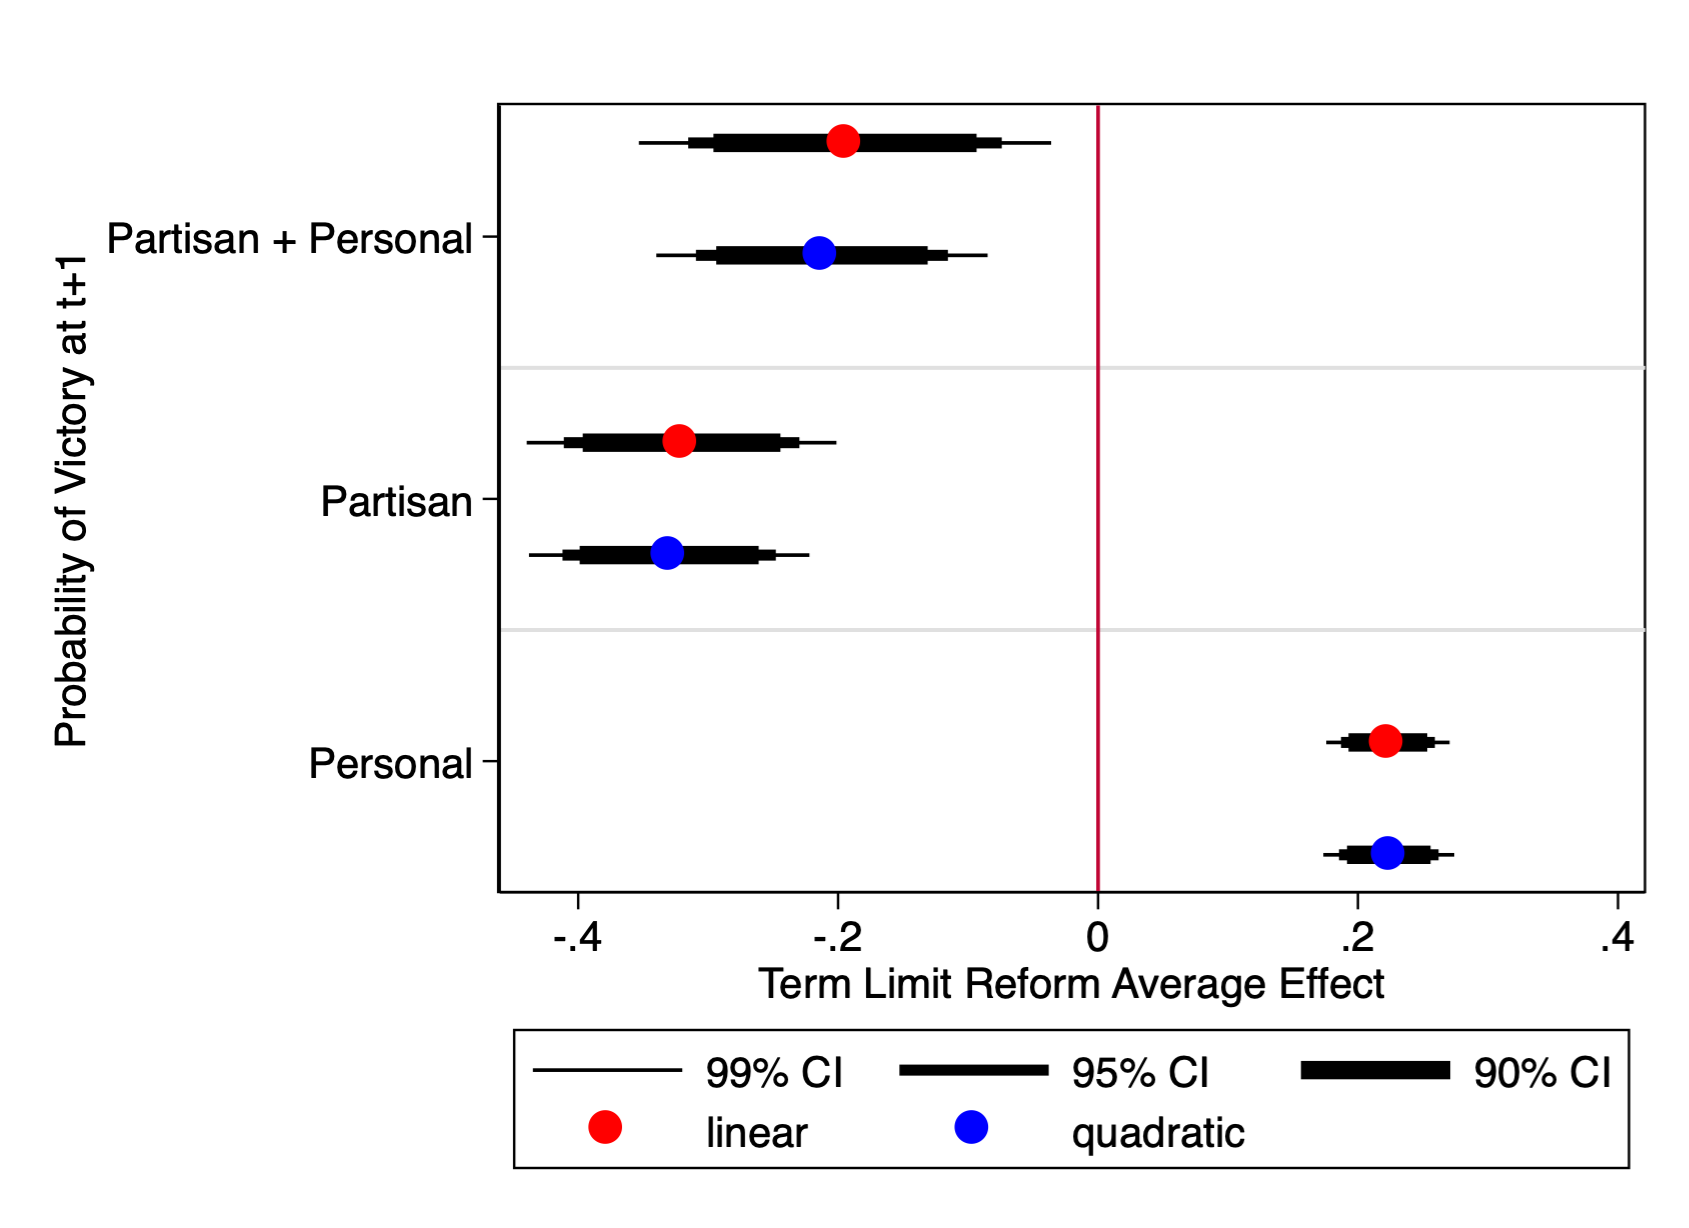
\includegraphics[width=0.9\textwidth]{../Figures/partisan_personal_inc_advantage.png}
       \captionsetup{justification=centering}
       
 \textbf{Note:} Figure \ref{fig:personal_vs_partisan} shows the average treatment effect of the Term Limit Reform on the probability of winning in the following election using a difference in discontinuity of close elections design. This average effect was estimated using the IW estimators following \citet{abraham_sun_2020} for each lead and lag relative to the first year a municipality implemented reelection. Optimal bandwidths following \citet{calonicoetal_2014} are used. This analysis identifies the party that wins at $t-1$ and studies the effect of this party barely winning (or losing) at $t$ on outcomes at election $t+1$ following \citet{klasnja_titiunik_2017}. I follow \citet{fowler_hall_2014} to decompose the incumbency advantage into the partisan and personal component. Red and blue points show that parallel trends hold, while hollow ones imply pretrends. 
\end{figure}  

\clearpage

\subsection{Identification assumptions}

To validate causal effects three identification assumptions need to hold. First, cohort weighted specifications need to show parallel trends for both incumbency advantage measures. As seen in Table \ref{tab:incumbency_wpolynomials}  this is the case. Cohort weights further assure that parallel trends are not spurious due to correlation between the $k$ period indicators relative to treatment implementation. Second, no anticipatory behavior from municipalities should be found; since we are only taking into account one election cycle post-treatment, we don't anticipate incumbents reacting in such a short time window. %[MISSING]%this is the case when running an ``event-to-event" analysis following \citet{cengiz_etal_2019}: there is no clustering in estimated coefficients on early and late state adopters.\footnote{Results available upon request.} 
Third, the design would be invalid if parties could manipulate close elections and sort themselves to those that imply a higher probability of winning. Two tests are commonly used to show validity on the design: (a) no covariate jump at the discontinuity on relevant pre-treatment variables and (b) density tests to see whether the number of municipalities above (or below) the cutoff threshold is significantly different from the number of municipalities below (or above). Appendix Figure \ref{tab:incumbency_wpolynomials_pop} showes evidence of no significant jump at the discontinuity of municipal population.\footnote{Next iteration of this working paper will include validation on municipal GDP, revenue and expenditures, geographic location and previous victory.} Furthermore, Appendix Figure \ref{fig:mccrary} shows no density difference between municipalities just above and below the cutoff.\footnote{Given the reduction in sample size from Table \ref{tab:abraham_sun_lagdv} to Table \ref{tab:incumbency_wpolynomials} one could have a concern that main results no longer hold in this close election setting. Appendix Table \ref{tab:abraham_sun_local} shows this is not the case by estimating results of Table \ref{tab:abraham_sun_lagdv} using as sample only the municipalities of the sample of Table \ref{tab:incumbency_wpolynomials}.}   

Overall, results show the Term Limit Removal Reform increased incumbent probability of winning at future elections. If this is the case, then we should expect a decrease in the effort placed by security forces in the country, especially from the party in government, the PRI. Federal forces, particularly the military in charge of tackling DTOs, should decrease the amount of narcotic crackdowns and seizures. Furthermore, this should generate a downward effect to local proxies, i.e. mayors in charge of tackling down local crime. In fact, this is what I find. 
   \clearpage

\section{Robustness}


\begin{table}[htbp]\def\sym#1{\ifmmode^{#1}\else\(^{#1}\)\fi}
\centering
\caption{Event-in-Discontinuity in close elections model: Effect of 2014 Term Limit Reform on Incumbency Advantage}
\label{tab:incumbency_wpolynomials}
\scalebox{0.8}{
\begin{tabular}{lcc}
\hline \hline
\\ \multicolumn{3}{l}{Dependent variable:}\\
& \multicolumn{1}{c}{Incumbent at t-1 won at t+1}  & \multicolumn{1}{c}{Incumbent at t won at t+1} \\
& \multicolumn{1}{c}{(indicator)}  & \multicolumn{1}{c}{(indicator)} \\
& \multicolumn{1}{c}{(1)} & \multicolumn{1}{c}{(2)}  \\
\cmidrule(lrr){2-2}  \cmidrule(lrr){3-3} \\
\addlinespace
& \multicolumn{2}{c}{linear polynomial} \\
\cmidrule(lrr){2-3} \\
4 Elections prior &       $ -0.0006^{} $ &       $ 0.0578^{*} $  \\
& ($ 0.0681 $ ) & ($ 0.0320 $ ) \\
3 Elections prior &       $ 0.0747^{} $ &        $ -0.1118^{***} $ \\
& ($ 0.1660 $ ) & ($ 0.0343 $ ) \\
2 Elections prior &          $ 0.1262^{} $ &       $ 0.0773^{} $ \\
& ($ 0.0965 $ ) & ($ 0.1420 $ ) \\
Election after Reform &         $ -0.0025^{} $ &        $ 0.1355^{***} $ \\
& ($     . $ ) & ($     . $ ) \\
Observations          &              2,002     &              3,084 \\
R-squared        &          0.5605   &          0.5887 \\
\\
& \multicolumn{2}{c}{quadratic polynomial} \\
\cmidrule(lrr){2-3} \\
4 Elections prior &       $ -0.1093^{***} $ &       $ 0.0657^{} $  \\
& ($ 0.0144 $ ) & ($ 0.0433 $ ) \\
3 Elections prior &       $ 0.3221^{***} $ &        $ -0.2892^{***} $ \\
& ($ 0.0608 $ ) & ($ 0.0557 $ ) \\
2 Elections prior &          $ 0.0467^{} $ &       $ 0.0358^{} $ \\
& ($ 0.0801 $ ) & ($ 0.1267 $ ) \\
Election after Reform &         $ -0.1600^{***} $ &        $ 0.1111^{***} $ \\
& ($     . $ ) & ($     . $ ) \\
Observations          &              2,766     &              4,038 \\
R-squared        &          0.5478   &          0.4066 \\
\\
Mun. FEs        &     \checkmark         &  \checkmark   \\
Year. FEs     &     \checkmark         &  \checkmark  \\
Controls$^a$  &    \checkmark     &       \checkmark \\
Cohort weighted  &         \checkmark &         \checkmark \\
\hline \hline
\multicolumn{3}{p{0.9\textwidth}}{\footnotesize{Notes: Coefficients show IW estimators following \citet{abraham_sun_2020}. Two relative time periods (lag 6 and 1) are removed to avoid collinearity problems noted by \citet{abraham_sun_2020} or because they are collinear or inexistent, like lag time period 2. Standard errors in parentheses are clustered at the state level for estimates in saturaded model. Significance-level: $^{***}$ 1\%; $^{**}$ 5\%; and $^*$ 10\%, that refer to two-sided t-test with the null hypothesis equal to 0 for each relative time period. $^a$ State-level controls include governor winning margin in last pre-treatment election and an indicator of whether the governor's party is the same as the federal incumbent party. Logged homicides per capita at the municipality level are also included as controls.}} \\
\end{tabular}
}
\end{table}
   
   
 \begin{figure}[H]   
\centering
 \caption{Effect of Term Limit Reform on Partisan and Personal Incumbency Advantage \\ -difference-in-discontinuity of close elections-}
 \label{fig:parallel_trend}
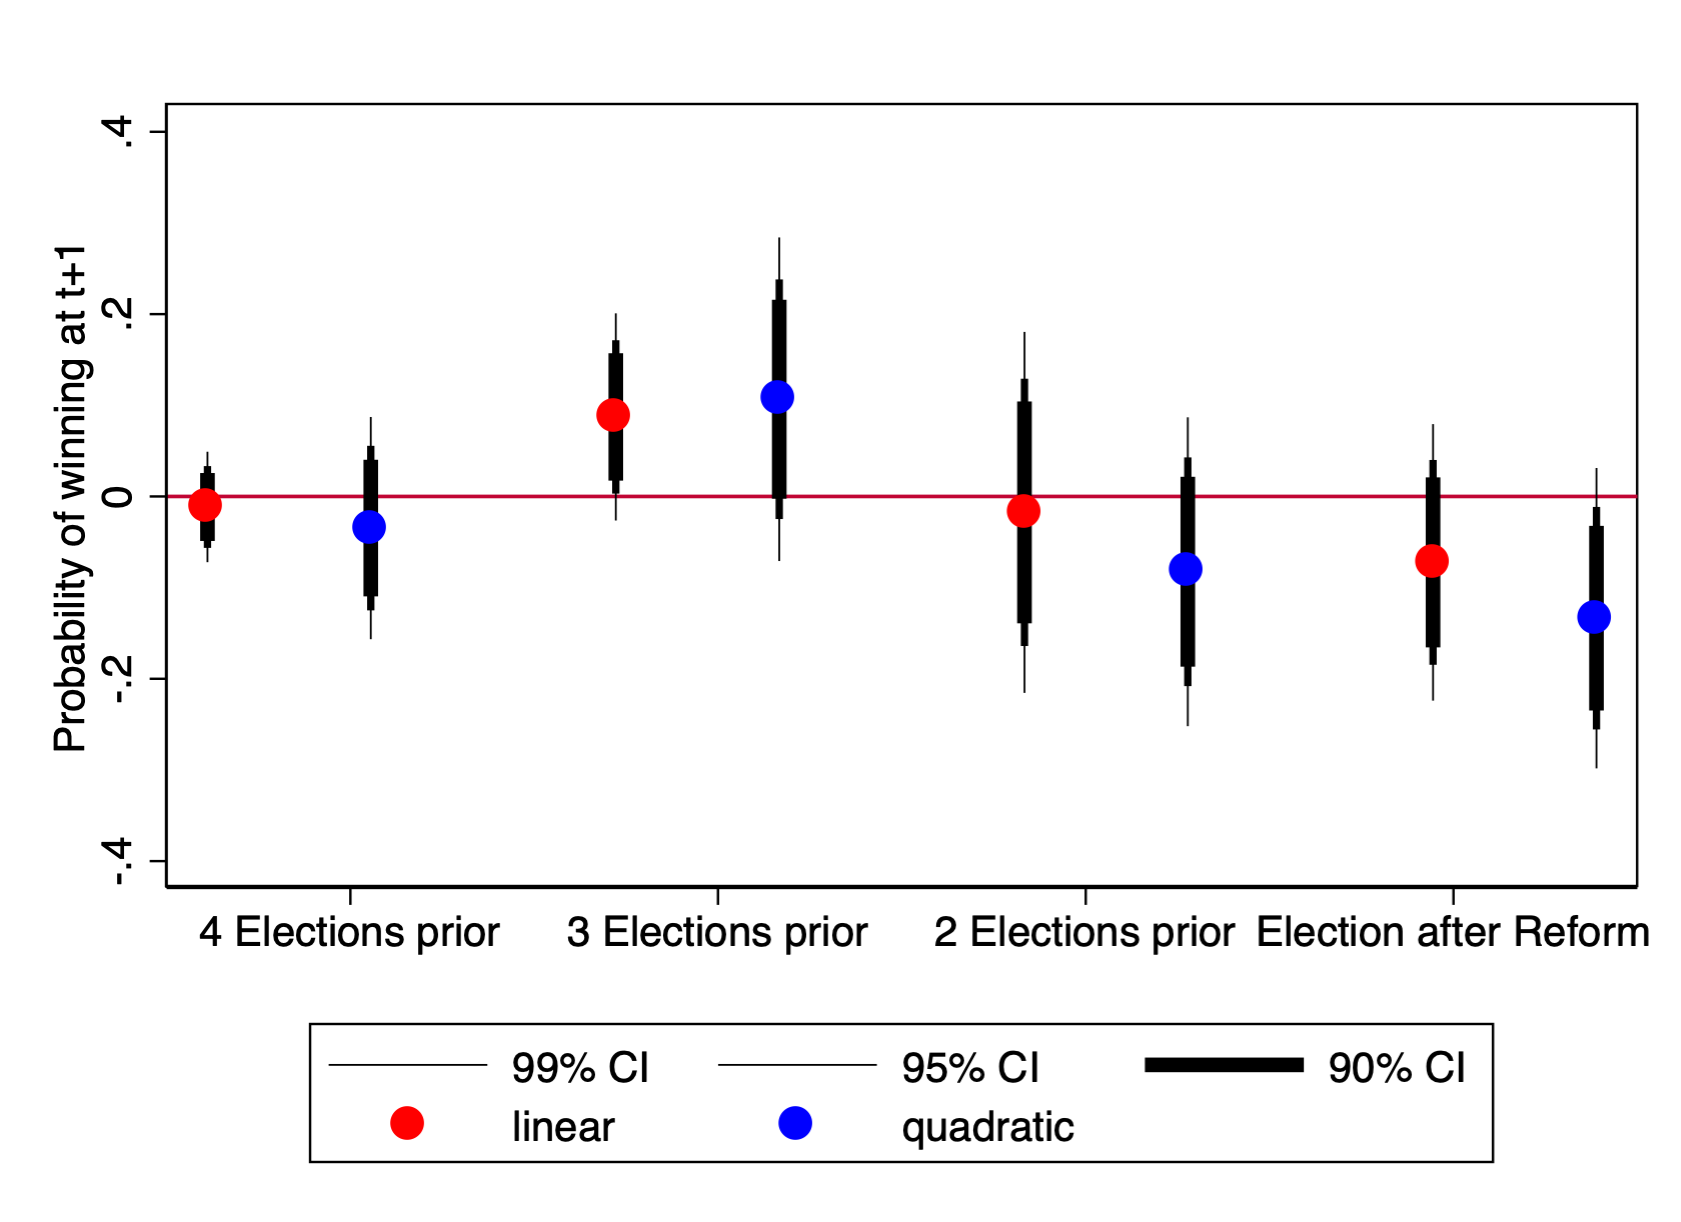
\includegraphics[width=0.9\textwidth]{../Figures/parallel_trends_incumbency.png}
       \captionsetup{justification=centering}
         
 \textbf{Note:} Figure \ref{fig:parallel_trend} shows the average treatment effect of the Term Limit Reform on the probability of winning in the following election using a difference in discontinuity of close elections design. This average effect was estimated using the IW estimators following \citet{abraham_sun_2020} for each lead and lag relative to the first year a municipality implemented reelection. Optimal bandwidths following \citet{calonicoetal_2014} are used. This analysis identifies the party that wins at $t-1$ and studies the effect of this party barely winning (or losing) at $t$ on outcomes at election $t+1$ following \citet{klasnja_titiunik_2017}.  
 
\end{figure}  


 \begin{figure}[H]   
\centering
 \caption{McCrary Test}
 \label{fig:mcrary}
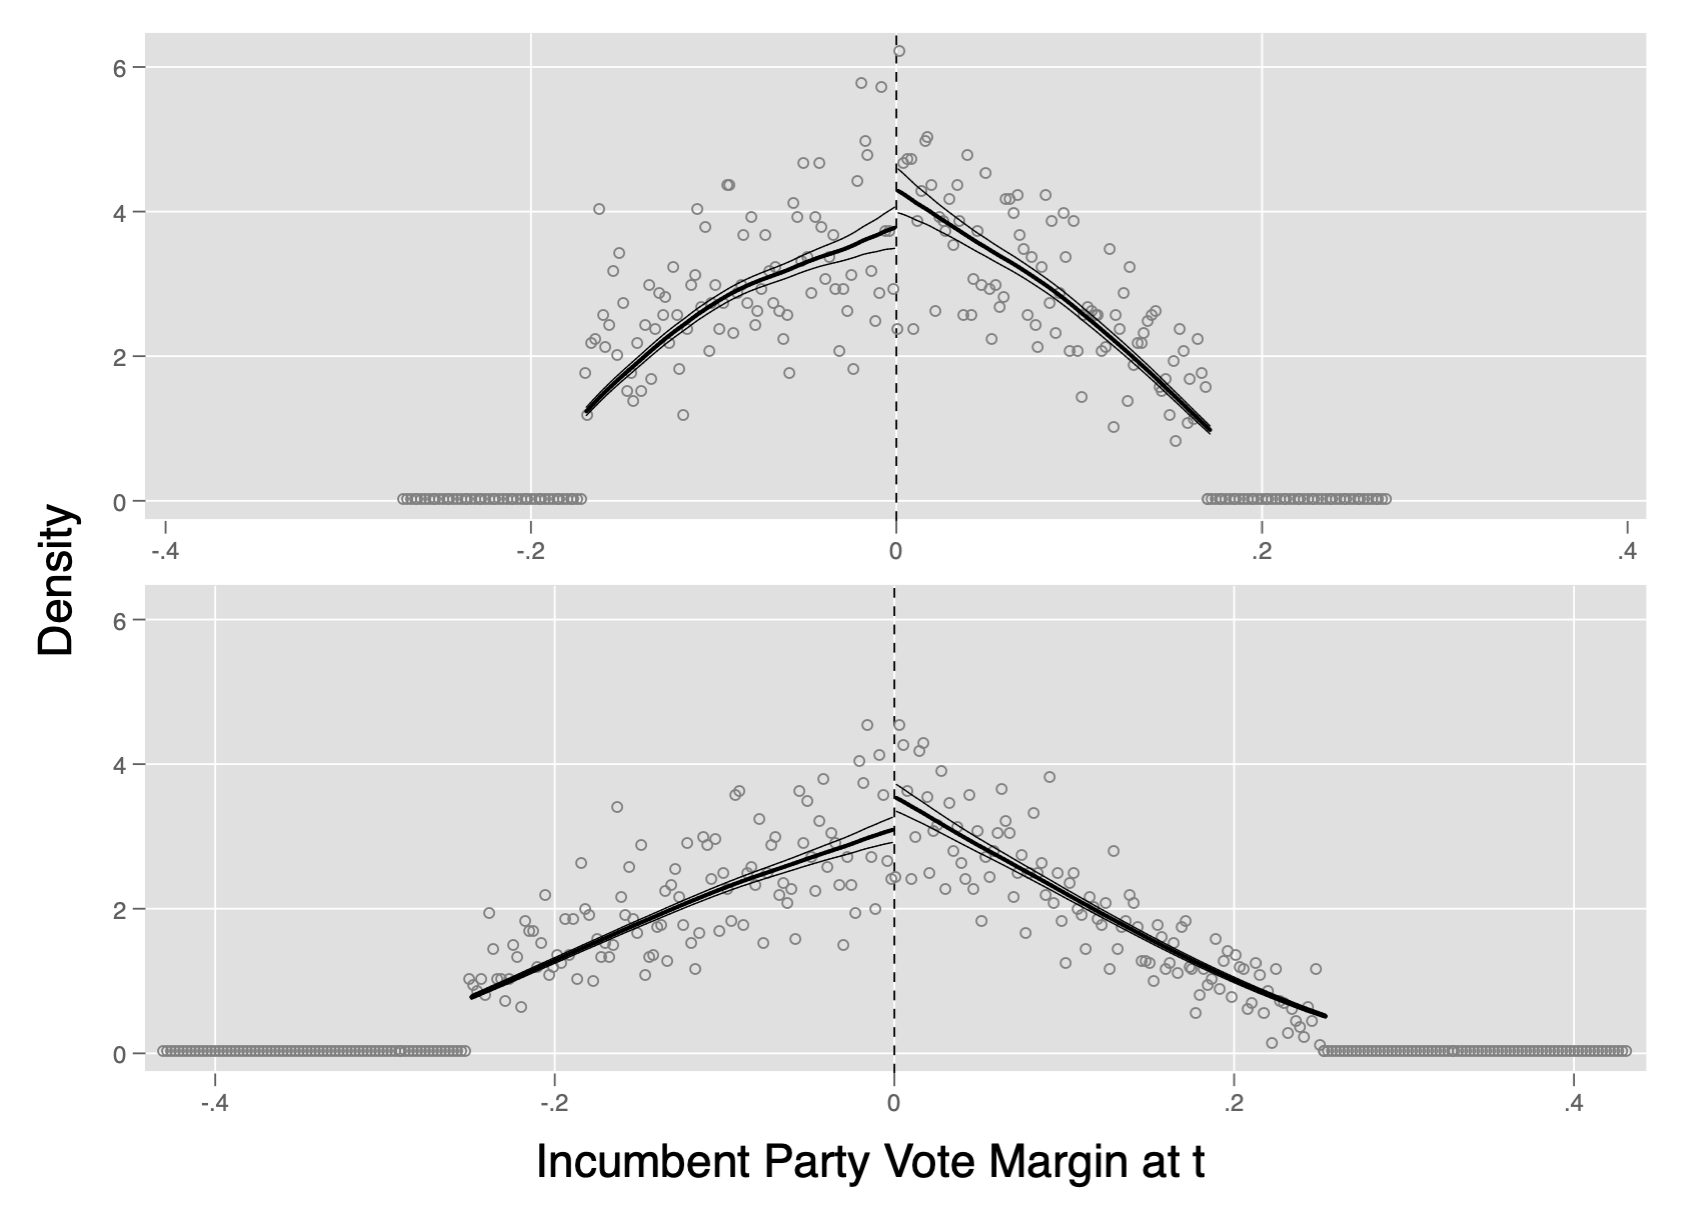
\includegraphics[width=0.9\textwidth]{../Figures/conditional_mccrary_test_pol1_final.png}
       \captionsetup{justification=centering}
         
 \textbf{Note:} 95\% confidence intervals reported. With 90\% levels confidence intervals overlap..  
 
\end{figure} 

 \begin{figure}[H]   
\centering
 \caption{No discontinuous jump of covariates}
 \label{fig:parallel_trend}
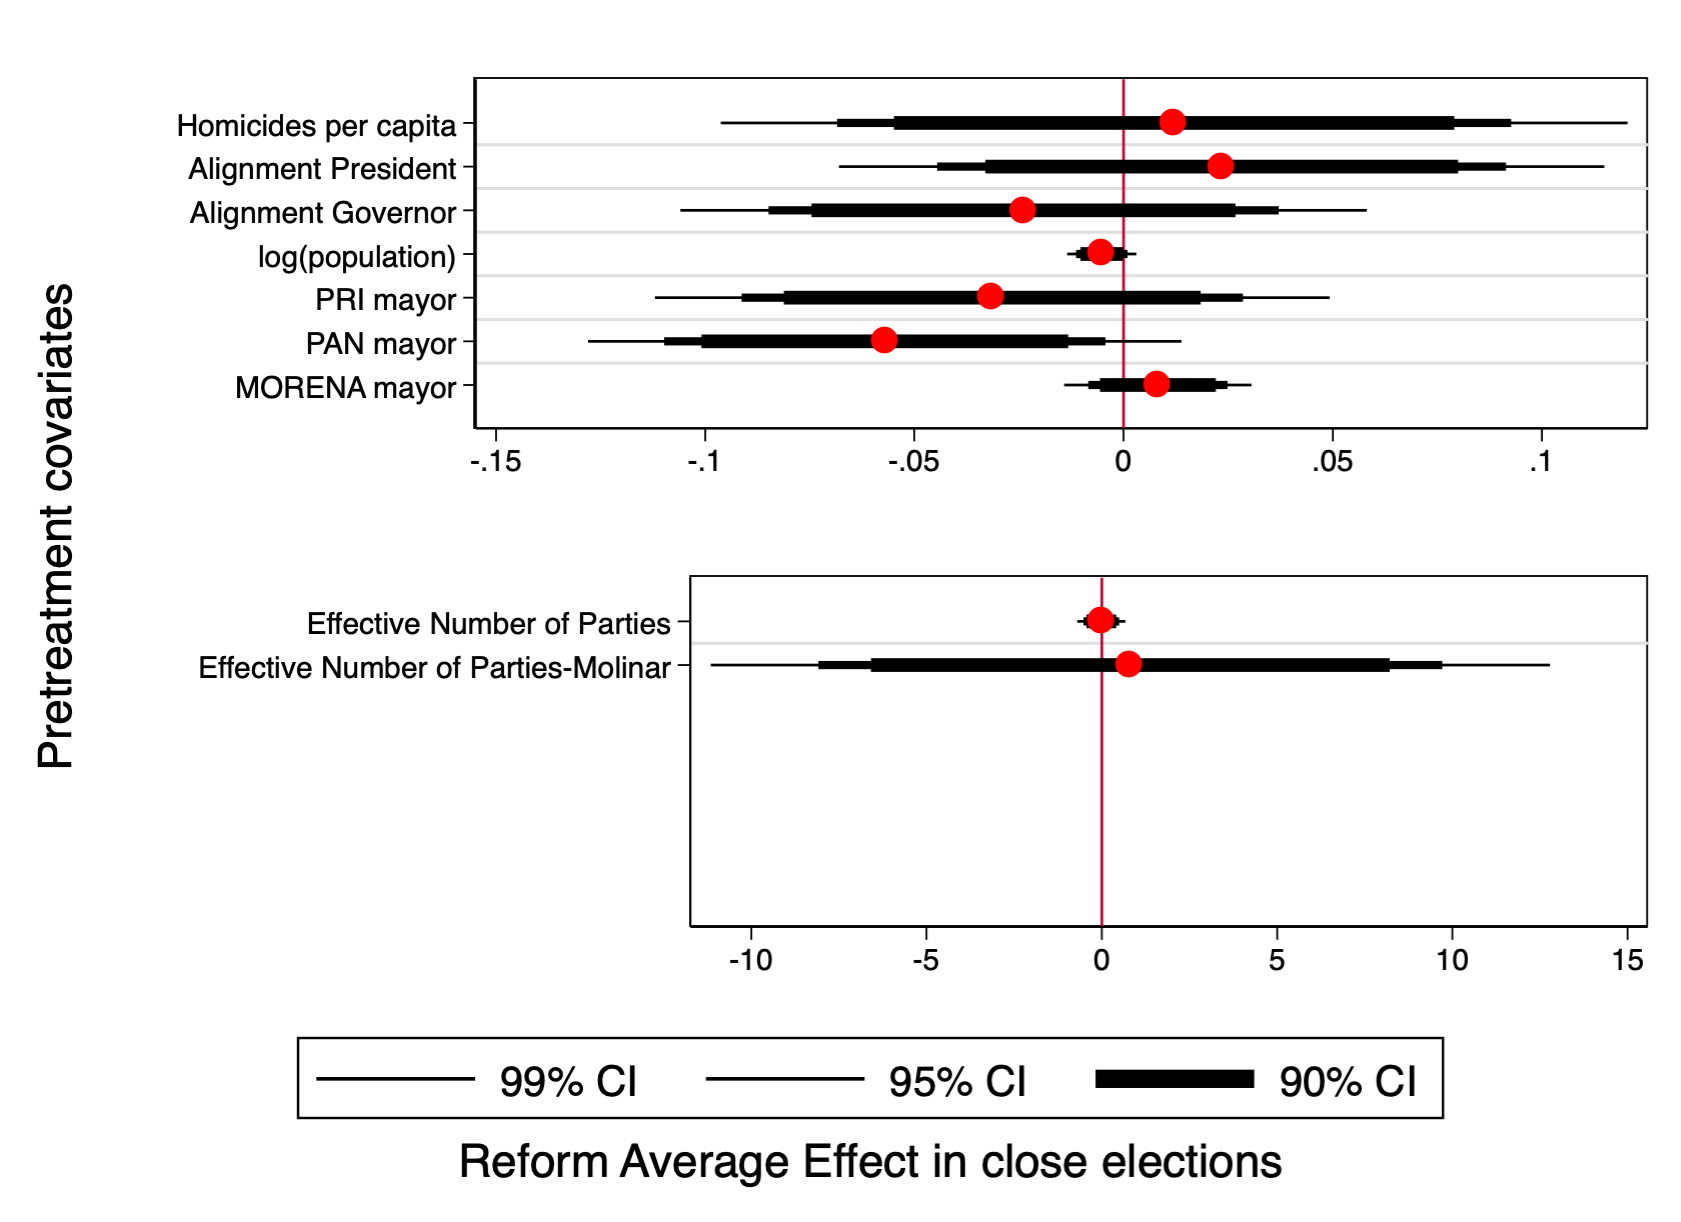
\includegraphics[width=0.9\textwidth]{../Figures/nojump.png}
       \captionsetup{justification=centering}
    
 %\textbf{Note:}.  
   
\end{figure} 


 \begin{figure}[H]   
\centering
 \caption{Testing Different Bandwidths}
 \label{fig:parallel_trend}
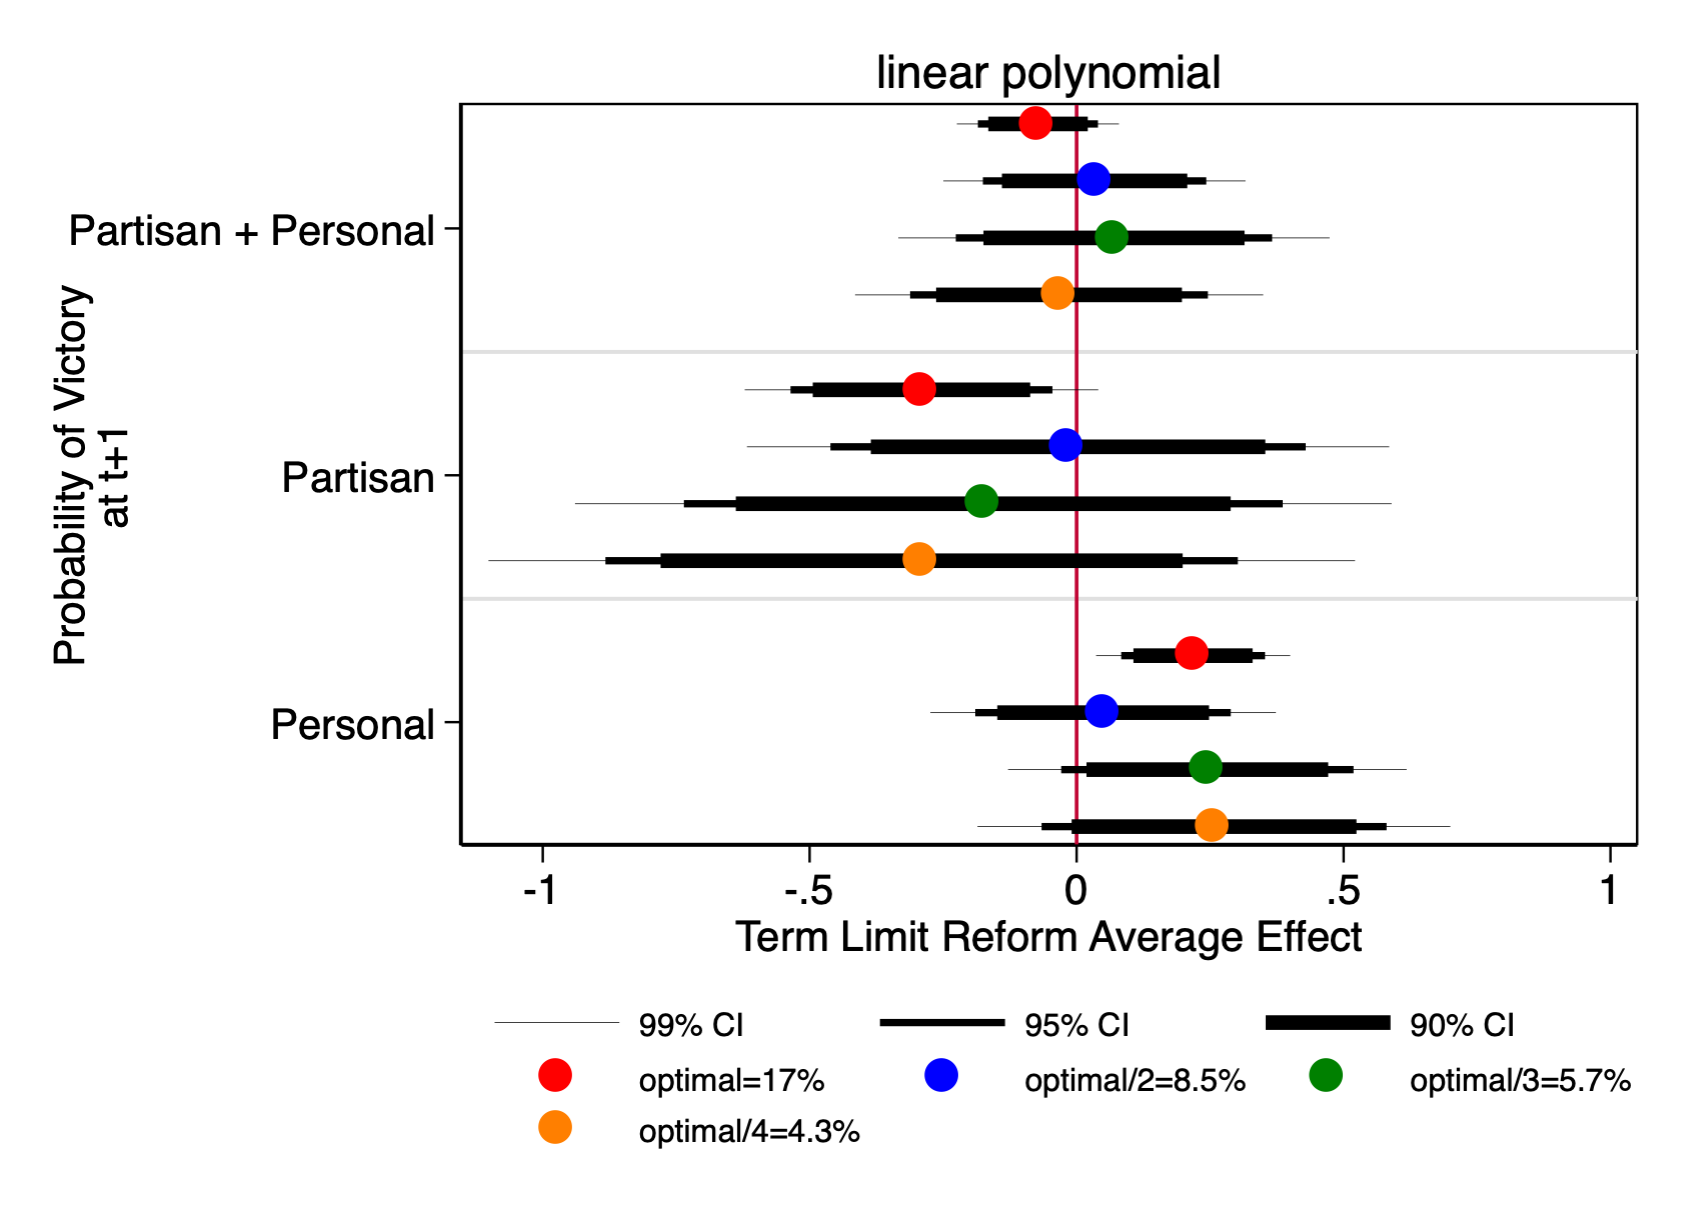
\includegraphics[width=0.9\textwidth]{../Figures/many_bandwidths_linear.png}
       \captionsetup{justification=centering}
 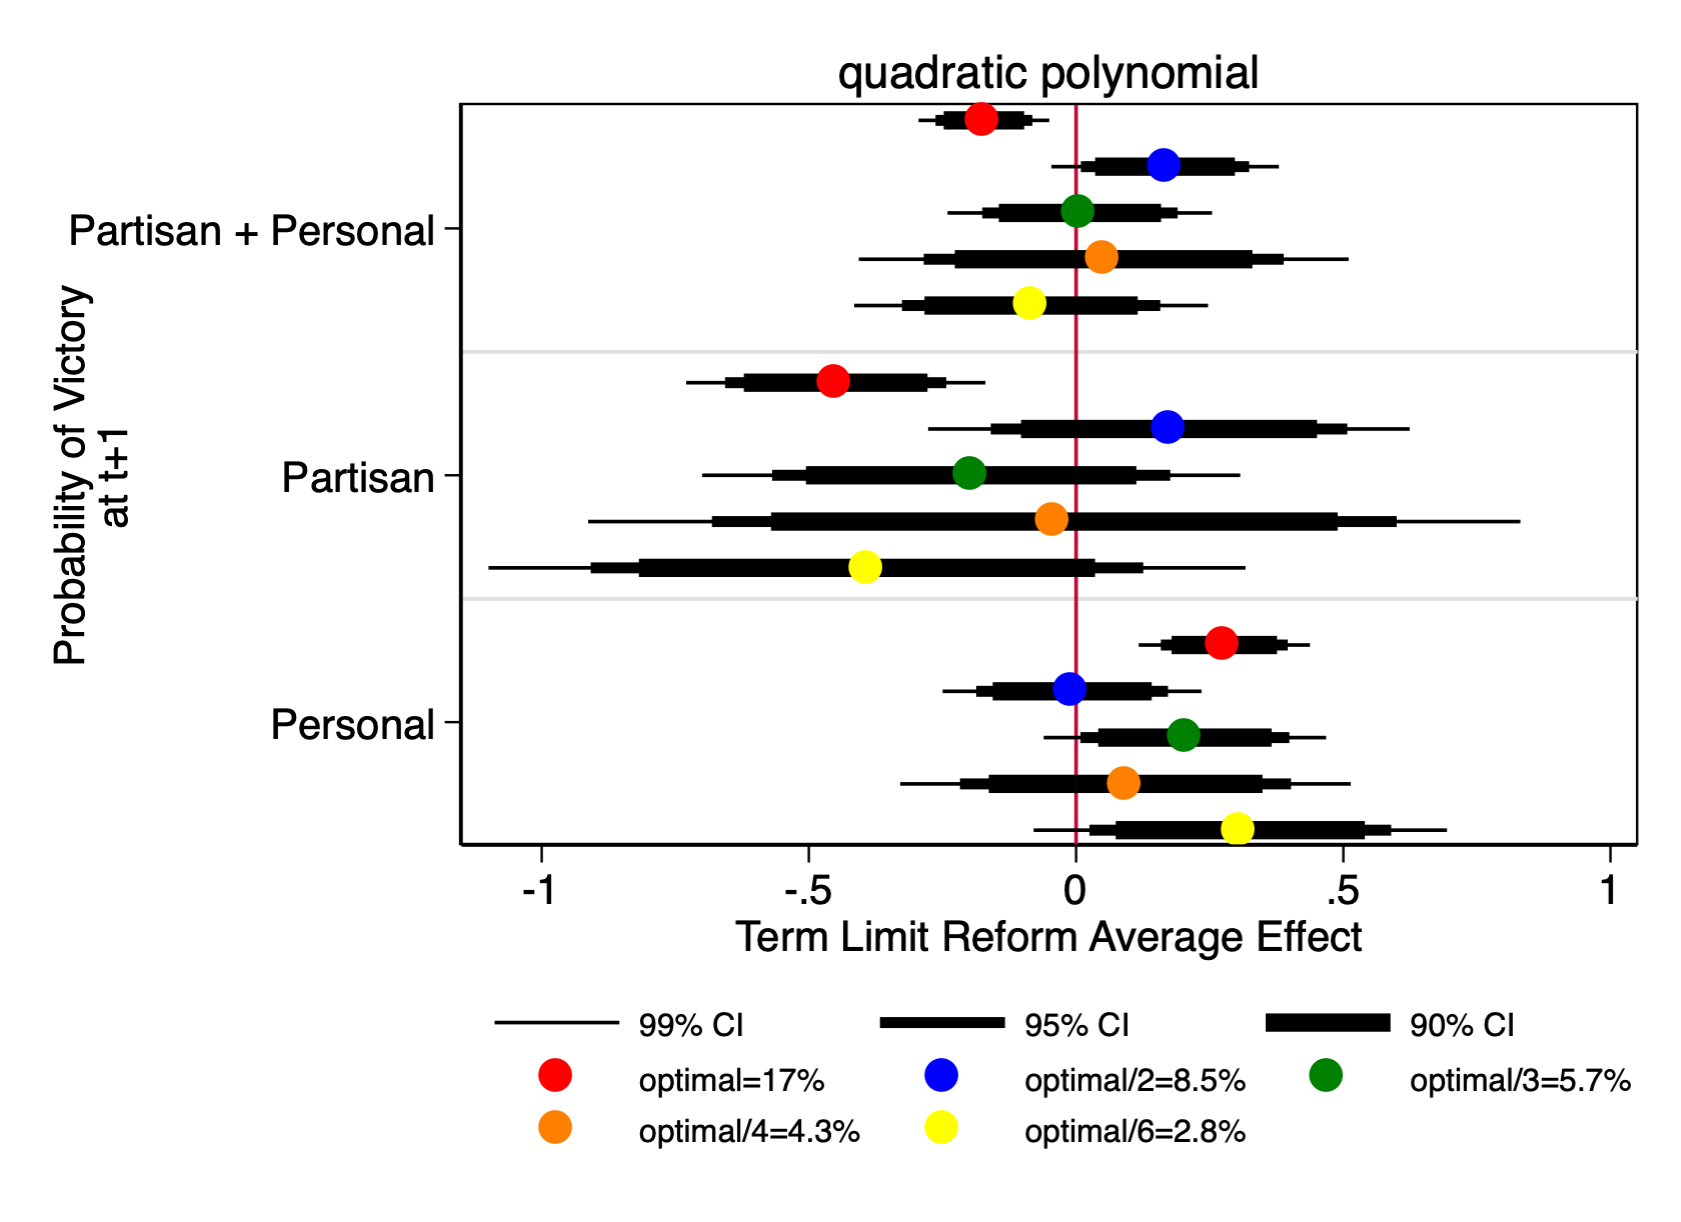
\includegraphics[width=0.9\textwidth]{../Figures/many_bandwidths_quadratic.png}

 %\textbf{Note:}.  
   
\end{figure} 



\clearpage

\section{Mechanisms}

\clearpage

\section{Conclusion} 

            
%APPENDIX -----------------------------------------------

%%%%%%%%%%%%
\bibliographystyle{aer} 
\bibliography{References}    

\clearpage
%APPENDIX -----------------------------------------------
\begin{appendix}
\renewcommand{\thetable}{A-\arabic{table}}
\setcounter{table}{0}
 
\renewcommand{\thefigure}{B-\arabic{figure}}
\setcounter{figure}{0}

   
%%%%%%%%%%%%%%%%%%%%%%%%%%%%%%%%% 

%%%% RDD design
\section{Regression Discontinuity Design of close elections, before and after the Term Limit Removal Reform of 2014 \label{appendix:rdd}} 

I begin by visualizing the effect of the reform on incumbency advantage.  Figure \ref{fig:incumbency_advantage} presents the RDD estimate of close elections on incumbency advantage  within an optimal bandwidth distance $h$ from the cutoff (0), and a quadratic polynomial:\footnote{A triangular kernel is used. Results are almost unchanged when using other polynomial functional forms.} Panel A shows a comparison of municipalities with incumbents at $t-1$ that barely won to those that barely lost in $t$ on the probability of electoral victory at $t+1$,\footnote{Incumbency advantage measure following \citet{klasnja_titiunik_2017}.} taking into account all elections from 1979 to 2014 (i.e. prior to the term-limit reform); Panel B shows the same comparison but restricting the sample to municipalities that implemented reelection after 2014. I do not consider those municipal elections that after 2014 did not implement reelection. Table \ref{tab:rdd} shows RD estimates using multiple polynomial functional forms. Even though RD estimates are biased in this setting, especially for Panel B in Figure \ref{fig:incumbency_advantage} (and even columns in Table \ref{tab:rdd}) since in the presence of staggered treatment timing and heterogeneous treatment effects across cohorts are not causally interpretable since we are considering both early vs late adopters of the reform on the treated,\footnote{The next iteration of this working paper will show this proof in the Appendix for RD designs.} they provide a striking depiction of what occurred before and after the electoral reform. 


\begin{figure}[H]
\centering
\caption{Effect of Term Limit Reform of 2014 on Incumbency Advantage, quadratic polynomial}
  \label{fig:incumbency_advantage} 

	%{\textbf Figure A: quadratic polynomial}
 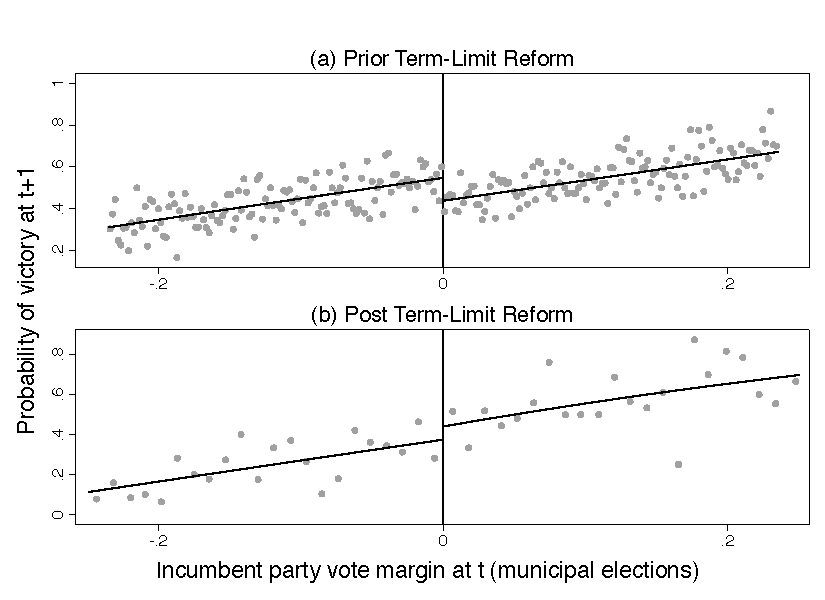
\includegraphics[width=1\textwidth]{../Figures_incumbency/RDD_incumbency_pol2.pdf}
     \captionsetup{justification=centering}  
       
\end{figure} 
       Note: Regression Discontinuity design of close elections on incumbency advantage. Panel (a) considers all elections from 1979 to 2014. Panel (b) considers all elections after 2014 for municipalities that implemented reelection.) 
\\
       
Before the reform, there was a negative statistical significant difference between municipalities that barely won and lost on the probability of success in the next election. This incumbency \emph{disadvantage} aligns strongly with a similar result found by \citet{klasnja_titiunik_2017} for the case of Mexico. \citet{klasnja_titiunik_2017} find that an incumbent party that is barely reelected suffers a reduction in the probability of winning the following election of 28 percentage points. In contrast, I find a reduction between 10.7 to 11.32 percentage points, a finding that considers 20 more years of elections since \citet{klasnja_titiunik_2017} cap their data from 1997 to 2009, while I consider elections since 1979 to 2014. 

More interesting is the finding that after reelection takes place the previous incumbency disadvantage disappears as noted by a positive and non-statistical significant difference between municipalities that barely lost and won an election. This initial RDD results provide suggestive evidence that the electoral reform generated an increase in the probability of victory in the next election for municipalities that barely won an election relative to those that barely lost. The next section addressed potential biases and presents robust findings of this same evidence.  


 \\ 
  
%Table:
\begin{table}[!htbp]\def\sym#1{\ifmmode^{#1}\else\(^{#1}\)\fi}
\caption{Regression Discontinuity Design of Close Elections on Incumbency Advantage, comparing pre and post-Term Limit Reform estimates}
\label{tab:rdd}
\begin{center} 
\scalebox{0.7}{
\begin{tabular}{lcccccccc}
 
\hline \hline   
\\
   
\multicolumn{9}{l}{Dependent variable:}\\
  
\\
            &\multicolumn{2}{c}{linear polynomial}      &\multicolumn{2}{c}{quadratic polynomial}   &\multicolumn{2}{c}{}                       &\multicolumn{2}{c}{}                       \\\cmidrule(lr){2-3}\cmidrule(lr){4-5}\cmidrule(lr){6-7}\cmidrule(lr){8-9}
            &\multicolumn{1}{c}{(1)}         &\multicolumn{1}{c}{(2)}         &\multicolumn{1}{c}{(3)}         &\multicolumn{1}{c}{(4)}         &\multicolumn{1}{c}{(5)}         &\multicolumn{1}{c}{(6)}         &\multicolumn{1}{c}{(7)}         &\multicolumn{1}{c}{(8)}         \\
\addlinespace
Conditional Probability of victory at t+1&      0.1138\sym{***}&      0.0640         &     -0.1074\sym{***}&      0.0724         &      0.1130\sym{***}&      0.0500         &     -0.1119\sym{***}&      0.0562         \\
            &    (0.0220)         &    (0.0711)         &    (0.0217)         &    (0.0635)         &    (0.0245)         &    (0.0863)         &    (0.0274)         &    (0.0845)         \\
\addlinespace
Observations&       8,026         &         711         &       8,622         &         888         &      11,255         &         897         &      10,125         &         956         \\
Post Reform (2014)&                     &  \checkmark         &                     &  \checkmark         &                     &  \checkmark         &                     &  \checkmark         \\
 
 
        
\hline \hline   
\multicolumn{9}{p{1.3\textwidth}}{\footnotesize{Notes: Standard errors in parentheses, with the following significance-level: $^{***}$ 1\%; $^{**}$ 5\%; and $^*$ 10\%, that refer to two-sided t-test. Optimal bandwidth following \citet{calonicoetal_2014} $^a$ Incumbency advantage measured following \citet{klasnja_titiunik_2017}. 
  }} \\  
\end{tabular}         
}
\end{center} 
\end{table} 

\clearpage


  
\end{document}
